\documentclass[]{book}
\usepackage{lmodern}
\usepackage{amssymb,amsmath}
\usepackage{ifxetex,ifluatex}
\usepackage{fixltx2e} % provides \textsubscript
\ifnum 0\ifxetex 1\fi\ifluatex 1\fi=0 % if pdftex
  \usepackage[T1]{fontenc}
  \usepackage[utf8]{inputenc}
\else % if luatex or xelatex
  \ifxetex
    \usepackage{mathspec}
  \else
    \usepackage{fontspec}
  \fi
  \defaultfontfeatures{Ligatures=TeX,Scale=MatchLowercase}
\fi
% use upquote if available, for straight quotes in verbatim environments
\IfFileExists{upquote.sty}{\usepackage{upquote}}{}
% use microtype if available
\IfFileExists{microtype.sty}{%
\usepackage{microtype}
\UseMicrotypeSet[protrusion]{basicmath} % disable protrusion for tt fonts
}{}
\usepackage[margin=1in]{geometry}
\usepackage{hyperref}
\hypersetup{unicode=true,
            pdftitle={EigenGWAS theory and application},
            pdfauthor={Guo-Bo Chen {[}chen.guobo@foxmail.com{]}},
            pdfborder={0 0 0},
            breaklinks=true}
\urlstyle{same}  % don't use monospace font for urls
\usepackage{natbib}
\bibliographystyle{apalike}
\usepackage{color}
\usepackage{fancyvrb}
\newcommand{\VerbBar}{|}
\newcommand{\VERB}{\Verb[commandchars=\\\{\}]}
\DefineVerbatimEnvironment{Highlighting}{Verbatim}{commandchars=\\\{\}}
% Add ',fontsize=\small' for more characters per line
\usepackage{framed}
\definecolor{shadecolor}{RGB}{248,248,248}
\newenvironment{Shaded}{\begin{snugshade}}{\end{snugshade}}
\newcommand{\AlertTok}[1]{\textcolor[rgb]{0.94,0.16,0.16}{#1}}
\newcommand{\AnnotationTok}[1]{\textcolor[rgb]{0.56,0.35,0.01}{\textbf{\textit{#1}}}}
\newcommand{\AttributeTok}[1]{\textcolor[rgb]{0.77,0.63,0.00}{#1}}
\newcommand{\BaseNTok}[1]{\textcolor[rgb]{0.00,0.00,0.81}{#1}}
\newcommand{\BuiltInTok}[1]{#1}
\newcommand{\CharTok}[1]{\textcolor[rgb]{0.31,0.60,0.02}{#1}}
\newcommand{\CommentTok}[1]{\textcolor[rgb]{0.56,0.35,0.01}{\textit{#1}}}
\newcommand{\CommentVarTok}[1]{\textcolor[rgb]{0.56,0.35,0.01}{\textbf{\textit{#1}}}}
\newcommand{\ConstantTok}[1]{\textcolor[rgb]{0.00,0.00,0.00}{#1}}
\newcommand{\ControlFlowTok}[1]{\textcolor[rgb]{0.13,0.29,0.53}{\textbf{#1}}}
\newcommand{\DataTypeTok}[1]{\textcolor[rgb]{0.13,0.29,0.53}{#1}}
\newcommand{\DecValTok}[1]{\textcolor[rgb]{0.00,0.00,0.81}{#1}}
\newcommand{\DocumentationTok}[1]{\textcolor[rgb]{0.56,0.35,0.01}{\textbf{\textit{#1}}}}
\newcommand{\ErrorTok}[1]{\textcolor[rgb]{0.64,0.00,0.00}{\textbf{#1}}}
\newcommand{\ExtensionTok}[1]{#1}
\newcommand{\FloatTok}[1]{\textcolor[rgb]{0.00,0.00,0.81}{#1}}
\newcommand{\FunctionTok}[1]{\textcolor[rgb]{0.00,0.00,0.00}{#1}}
\newcommand{\ImportTok}[1]{#1}
\newcommand{\InformationTok}[1]{\textcolor[rgb]{0.56,0.35,0.01}{\textbf{\textit{#1}}}}
\newcommand{\KeywordTok}[1]{\textcolor[rgb]{0.13,0.29,0.53}{\textbf{#1}}}
\newcommand{\NormalTok}[1]{#1}
\newcommand{\OperatorTok}[1]{\textcolor[rgb]{0.81,0.36,0.00}{\textbf{#1}}}
\newcommand{\OtherTok}[1]{\textcolor[rgb]{0.56,0.35,0.01}{#1}}
\newcommand{\PreprocessorTok}[1]{\textcolor[rgb]{0.56,0.35,0.01}{\textit{#1}}}
\newcommand{\RegionMarkerTok}[1]{#1}
\newcommand{\SpecialCharTok}[1]{\textcolor[rgb]{0.00,0.00,0.00}{#1}}
\newcommand{\SpecialStringTok}[1]{\textcolor[rgb]{0.31,0.60,0.02}{#1}}
\newcommand{\StringTok}[1]{\textcolor[rgb]{0.31,0.60,0.02}{#1}}
\newcommand{\VariableTok}[1]{\textcolor[rgb]{0.00,0.00,0.00}{#1}}
\newcommand{\VerbatimStringTok}[1]{\textcolor[rgb]{0.31,0.60,0.02}{#1}}
\newcommand{\WarningTok}[1]{\textcolor[rgb]{0.56,0.35,0.01}{\textbf{\textit{#1}}}}
\usepackage{longtable,booktabs}
\usepackage{graphicx,grffile}
\makeatletter
\def\maxwidth{\ifdim\Gin@nat@width>\linewidth\linewidth\else\Gin@nat@width\fi}
\def\maxheight{\ifdim\Gin@nat@height>\textheight\textheight\else\Gin@nat@height\fi}
\makeatother
% Scale images if necessary, so that they will not overflow the page
% margins by default, and it is still possible to overwrite the defaults
% using explicit options in \includegraphics[width, height, ...]{}
\setkeys{Gin}{width=\maxwidth,height=\maxheight,keepaspectratio}
\IfFileExists{parskip.sty}{%
\usepackage{parskip}
}{% else
\setlength{\parindent}{0pt}
\setlength{\parskip}{6pt plus 2pt minus 1pt}
}
\setlength{\emergencystretch}{3em}  % prevent overfull lines
\providecommand{\tightlist}{%
  \setlength{\itemsep}{0pt}\setlength{\parskip}{0pt}}
\setcounter{secnumdepth}{5}
% Redefines (sub)paragraphs to behave more like sections
\ifx\paragraph\undefined\else
\let\oldparagraph\paragraph
\renewcommand{\paragraph}[1]{\oldparagraph{#1}\mbox{}}
\fi
\ifx\subparagraph\undefined\else
\let\oldsubparagraph\subparagraph
\renewcommand{\subparagraph}[1]{\oldsubparagraph{#1}\mbox{}}
\fi

%%% Use protect on footnotes to avoid problems with footnotes in titles
\let\rmarkdownfootnote\footnote%
\def\footnote{\protect\rmarkdownfootnote}

%%% Change title format to be more compact
\usepackage{titling}

% Create subtitle command for use in maketitle
\newcommand{\subtitle}[1]{
  \posttitle{
    \begin{center}\large#1\end{center}
    }
}

\setlength{\droptitle}{-2em}

  \title{EigenGWAS theory and application}
    \pretitle{\vspace{\droptitle}\centering\huge}
  \posttitle{\par}
    \author{Guo-Bo Chen
{[}\href{mailto:chen.guobo@foxmail.com}{\nolinkurl{chen.guobo@foxmail.com}}{]}}
    \preauthor{\centering\large\emph}
  \postauthor{\par}
      \predate{\centering\large\emph}
  \postdate{\par}
    \date{2018-11-27}

\usepackage{booktabs}

\begin{document}
\maketitle

{
\setcounter{tocdepth}{1}
\tableofcontents
}
\hypertarget{eigengwas-basis}{%
\chapter{EigenGWAS basis}\label{eigengwas-basis}}

This project is dedicated to EigenGWAS, a linear model analysis approach
for eigenvectors on genomic data, which can be represented as
\(\mathbf{X}\) the \(n \times m\) genotype matrix. Without loss of
generality, \(x_j\) for the \(i^{th}\) locus is a biallic locus. The
data matrix \(\mathbf{X}\) can be generated from genotyping chips, NGS,
or GBS.

\begin{Shaded}
\begin{Highlighting}[]
\KeywordTok{set.seed}\NormalTok{(}\DecValTok{2018}\NormalTok{)}
\NormalTok{freq=}\KeywordTok{runif}\NormalTok{(}\DecValTok{1000}\NormalTok{, }\FloatTok{0.1}\NormalTok{, }\FloatTok{0.9}\NormalTok{)}
\NormalTok{X=}\KeywordTok{matrix}\NormalTok{(}\DecValTok{0}\NormalTok{, }\DecValTok{100}\NormalTok{, }\KeywordTok{length}\NormalTok{(freq))}
\ControlFlowTok{for}\NormalTok{(i }\ControlFlowTok{in} \DecValTok{1}\OperatorTok{:}\KeywordTok{length}\NormalTok{(freq)) \{}
\NormalTok{  X[,i]=}\KeywordTok{rbinom}\NormalTok{(}\KeywordTok{nrow}\NormalTok{(X), }\DecValTok{2}\NormalTok{, freq[i])}

\NormalTok{\}}
\KeywordTok{print}\NormalTok{(}\KeywordTok{dim}\NormalTok{(X))}
\CommentTok{## [1]  100 1000}
\KeywordTok{plot}\NormalTok{(freq, }\KeywordTok{colMeans}\NormalTok{(X)}\OperatorTok{/}\DecValTok{2}\NormalTok{, }\DataTypeTok{xlab=}\StringTok{"Simulated frequency"}\NormalTok{, }\DataTypeTok{ylab=}\StringTok{"Estimated frequency"}\NormalTok{, }\DataTypeTok{bty=}\StringTok{'n'}\NormalTok{, }\DataTypeTok{pch=}\DecValTok{16}\NormalTok{, }\DataTypeTok{cex=}\FloatTok{0.5}\NormalTok{)}
\KeywordTok{abline}\NormalTok{(}\DataTypeTok{a=}\DecValTok{0}\NormalTok{, }\DataTypeTok{b=}\DecValTok{1}\NormalTok{, }\DataTypeTok{col=}\StringTok{"red"}\NormalTok{, }\DataTypeTok{lty=}\DecValTok{2}\NormalTok{)}
\end{Highlighting}
\end{Shaded}

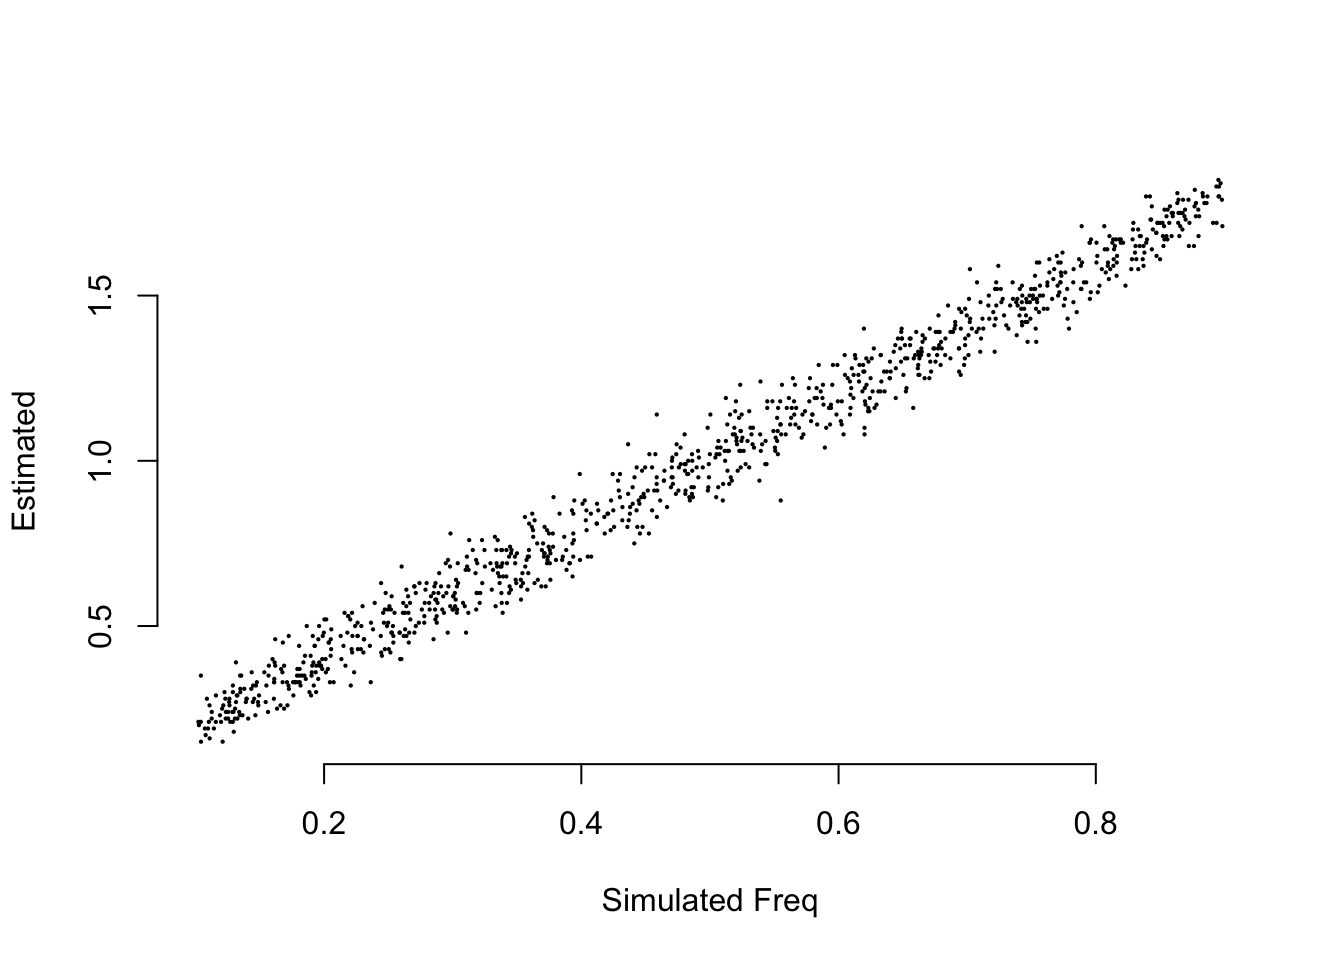
\includegraphics{EigenGWAS_files/figure-latex/x-1.pdf}

\hypertarget{genetic-relatedness-matrix-mathbfg}{%
\section{\texorpdfstring{Genetic relatedness matrix
\(\mathbf{G}\)}{Genetic relatedness matrix \textbackslash{}mathbf\{G\}}}\label{genetic-relatedness-matrix-mathbfg}}

We can construct the \(n\times\) genetic relatedness matrix as
\(\mathbf{X}\) the \(n\times m\) genotype matrix. We can construct the
\(n\times\) genetic relatedness matrix as

\[\mathbf{G}=\tilde{\mathbf{X}}\tilde{\mathbf{X}}^T\] in which
\(\tilde{\mathbf{X}}\) is the scaled form of \(\mathbf{X}\) However,
upon the mating type of the species, \(\mathbf{G}\) should be
constructly differently. For a random mating population, \(x_l\) is
scaled as \(\tilde{x}_l=\frac{x_l-2p_l}{\sqrt{2p_lq_l}}\), whereas for
inbred population, \(\tilde{x}_l=\frac{x_l-2p_l}{\sqrt{4p_lq_l}}\).
\(q_l\) equals \(1-p_l\).

So for a pair of individuals \(i\) and \(j\),
\[G_{ij}=\frac{1}{\tilde{m}}\sum_l^{\tilde{m}}\frac{(x_{il}-2p_l)(x_{jl}-2p_l)}{2(1+F)p_iq_i}\]
in which \(\tilde{m}\) is the number of genotyped loci at both individal
\(i\) and \(j\), and \(F\) the inbreeding coefficient takes value of 0
for random mating population and 1 for inbred population.

\hypertarget{statistical-properties-of-mathbfg}{%
\subsection{\texorpdfstring{Statistical properties of
\(\mathbf{G}\)}{Statistical properties of \textbackslash{}mathbf\{G\}}}\label{statistical-properties-of-mathbfg}}

Given \(\mathbf{G}\), we can define two population parameters, \(n_e\),
the effective population size, and \(m_e\), the effective number of
markers.

Let \(\mathbf{G}_o\) denote the off diagonal elements of \(\mathbf{G}\),
then we have \[n_e=\frac{-1}{mean(\mathbf{G}_o)}\] \(n_e\) reflects true
relatedness between any pair of samples;

\[m_e=\frac{1}{Var(\mathbf{G}_o)}\] The ratio between \(\frac{m_e}{m}\)
reflects general linkage disequilibrium between the markers.
Alternatively, \(m_e\) can be written as
\[m_e=\frac{\sum_{i=1}^m\sum_{j=1}^m\rho_{ij}}{m^2}\]

\begin{Shaded}
\begin{Highlighting}[]
\NormalTok{Xs=}\KeywordTok{apply}\NormalTok{(X, }\DecValTok{2}\NormalTok{, scale)}
\NormalTok{G=Xs }\OperatorTok\StringTok{ }\KeywordTok{t}\NormalTok{(Xs)}\OperatorTok{/}\KeywordTok{ncol}\NormalTok{(X)}
\NormalTok{Ne=}\OperatorTok{-}\DecValTok{1}\OperatorTok{/}\KeywordTok{mean}\NormalTok{(G[}\KeywordTok{col}\NormalTok{(G)}\OperatorTok{<}\KeywordTok{row}\NormalTok{(G)])}
\NormalTok{Me=}\DecValTok{1}\OperatorTok{/}\KeywordTok{var}\NormalTok{(G[}\KeywordTok{col}\NormalTok{(G)}\OperatorTok{<}\KeywordTok{row}\NormalTok{(G)])}
\KeywordTok{print}\NormalTok{(}\KeywordTok{paste}\NormalTok{(}\StringTok{"Ne="}\NormalTok{, Ne, }\StringTok{"Me="}\NormalTok{, Me, }\StringTok{"given N="}\NormalTok{, }\KeywordTok{nrow}\NormalTok{(Xs), }\StringTok{"and M="}\NormalTok{, }\KeywordTok{ncol}\NormalTok{(Xs)))}
\CommentTok{## [1] "Ne= 100 Me= 1080.91076380488 given N= 100 and M= 1000"}
\KeywordTok{hist}\NormalTok{(G[}\KeywordTok{col}\NormalTok{(G)}\OperatorTok{<}\KeywordTok{row}\NormalTok{(G)], }\DataTypeTok{main=}\StringTok{"GRM"}\NormalTok{, }\DataTypeTok{xlab=}\StringTok{"Relatedness"}\NormalTok{, }\DataTypeTok{breaks =} \DecValTok{25}\NormalTok{)}
\KeywordTok{legend}\NormalTok{(}\StringTok{"topright"}\NormalTok{, }\DataTypeTok{legend =} \KeywordTok{c}\NormalTok{(}\KeywordTok{paste0}\NormalTok{(}\StringTok{"Ne="}\NormalTok{, }\KeywordTok{format}\NormalTok{(Ne, }\DataTypeTok{digits =} \DecValTok{2}\NormalTok{)), }\KeywordTok{paste0}\NormalTok{(}\StringTok{"Me="}\NormalTok{, }\KeywordTok{format}\NormalTok{(Me, }\DataTypeTok{digits =} \DecValTok{2}\NormalTok{)) ), }\DataTypeTok{bty =} \StringTok{'n'}\NormalTok{)}
\end{Highlighting}
\end{Shaded}

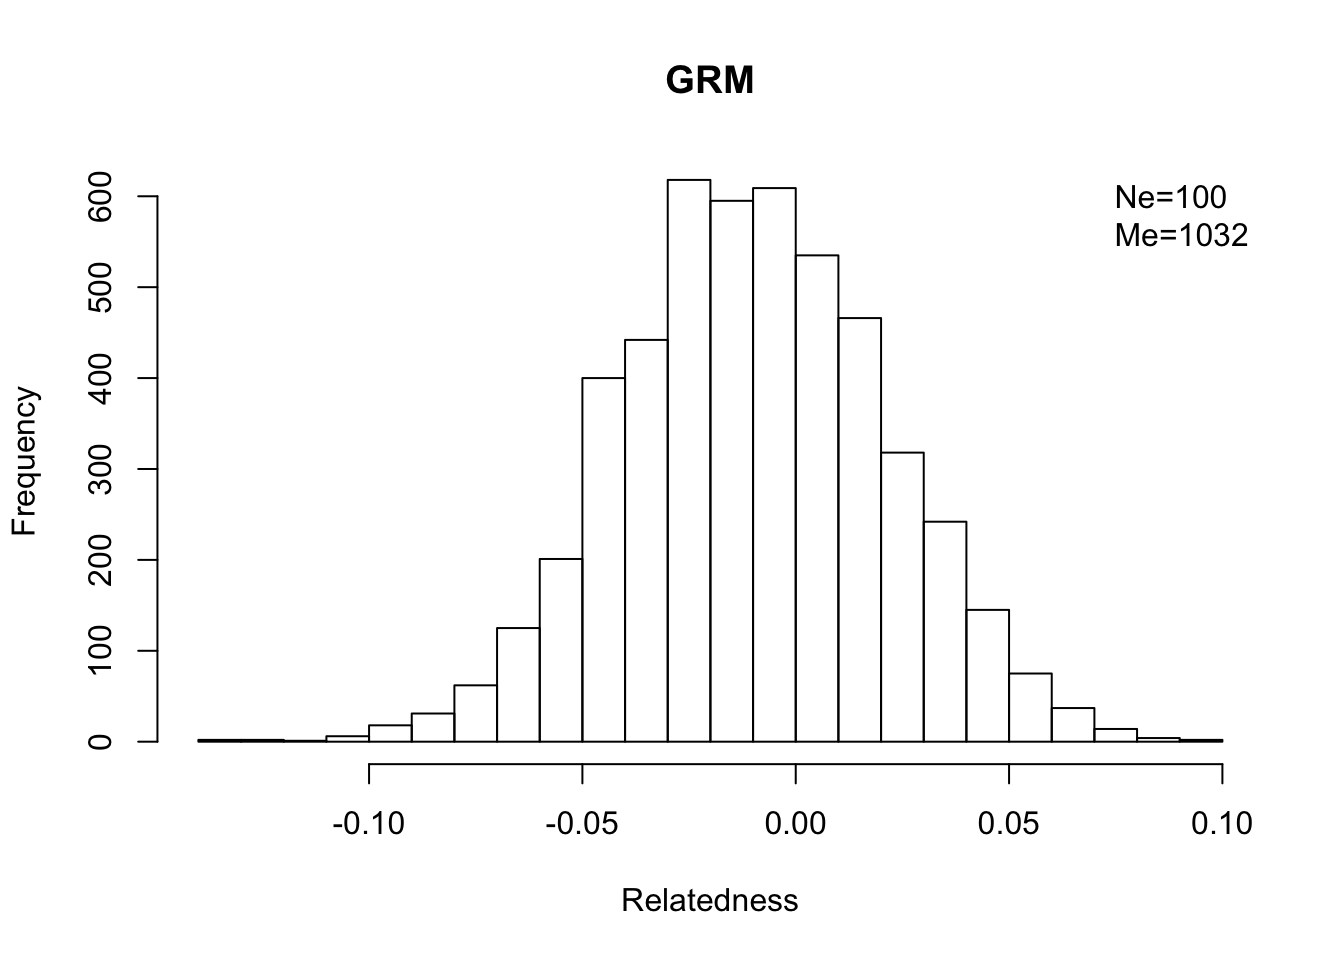
\includegraphics{EigenGWAS_files/figure-latex/G-1.pdf}

\hypertarget{eigengwas-analysis}{%
\section{EigenGWAS analysis}\label{eigengwas-analysis}}

Given eigenanalysis of \(\mathbf{X}\), we have \(\mathbf{E\Lambda E}\),
in which \(\mathbf{\Lambda}\) is the diagonal matrix for eigenvalues and
\(\mathbf{E}_k\) is the eigenvector associated with the \(k^{th}\)
largest eigenvalue, and regress \(\mathbf{E}_k\), the \(k^{th}\) column,
on each marker, we have the model below

\[\mathbf{E}_k=a+\beta_j\mathbf{x}_i+e\]

It consequently generates \(m\) estimates of \(\beta\), \(\sigma_j\),
and their corresponding \(p\) values. Given the \(m\) \(p\) values, the
conventional Manhattan plot can be made.

In particular, the one-degree-of-freedom \(\chi^2_1\) has approximation
as
\[4\frac{\color{red}{n_1}\color{blue}{n_2}}{n}\frac{(\color{red}{p_{1,l}}-\color{blue}{p_{2,l}})^2}{\bar{p}_l\bar{q}_l}\].
\(\color{red}{n_1}\) and \(\color{blue}{n_2}\) are the numbers of
samples at the left and right side of ``0'' on the eigenvector, see the
figure below. \(\color{red}{p_{1,l}}\) and \(\color{blue}{p_{2,l}}\) are
frequencies of the reference allele in two subgroups, respectively.
\(\bar{p_l}\) is the allele frequency of the reference allele.

\begin{Shaded}
\begin{Highlighting}[]
\NormalTok{eigenG=}\KeywordTok{eigen}\NormalTok{(G)}
\KeywordTok{layout}\NormalTok{(}\KeywordTok{matrix}\NormalTok{(}\DecValTok{1}\OperatorTok{:}\DecValTok{2}\NormalTok{, }\DecValTok{1}\NormalTok{, }\DecValTok{2}\NormalTok{))}
\KeywordTok{barplot}\NormalTok{(eigenG}\OperatorTok{$}\NormalTok{values, }\DataTypeTok{main=}\StringTok{"Eigenvalues"}\NormalTok{)}
\KeywordTok{plot}\NormalTok{(eigenG}\OperatorTok{$}\NormalTok{vectors[,}\DecValTok{1}\NormalTok{], eigenG}\OperatorTok{$}\NormalTok{vectors[,}\DecValTok{2}\NormalTok{], }\DataTypeTok{xlab=}\StringTok{"Eigen 1"}\NormalTok{, }\DataTypeTok{ylab=}\StringTok{"Eigen 2"}\NormalTok{, }\DataTypeTok{bty=}\StringTok{'n'}\NormalTok{, }\DataTypeTok{main=}\StringTok{"Eigenspace"}\NormalTok{, }\DataTypeTok{pch=}\DecValTok{16}\NormalTok{, }\DataTypeTok{cex=}\FloatTok{0.5}\NormalTok{, }\DataTypeTok{col=}\KeywordTok{ifelse}\NormalTok{(eigenG}\OperatorTok{$}\NormalTok{vectors[,}\DecValTok{1}\NormalTok{]}\OperatorTok{>}\DecValTok{0}\NormalTok{, }\StringTok{"red"}\NormalTok{, }\StringTok{"blue"}\NormalTok{))}
\KeywordTok{abline}\NormalTok{(}\DataTypeTok{v=}\DecValTok{0}\NormalTok{, }\DataTypeTok{col=}\StringTok{"grey"}\NormalTok{, }\DataTypeTok{lty=}\DecValTok{2}\NormalTok{)}
\end{Highlighting}
\end{Shaded}

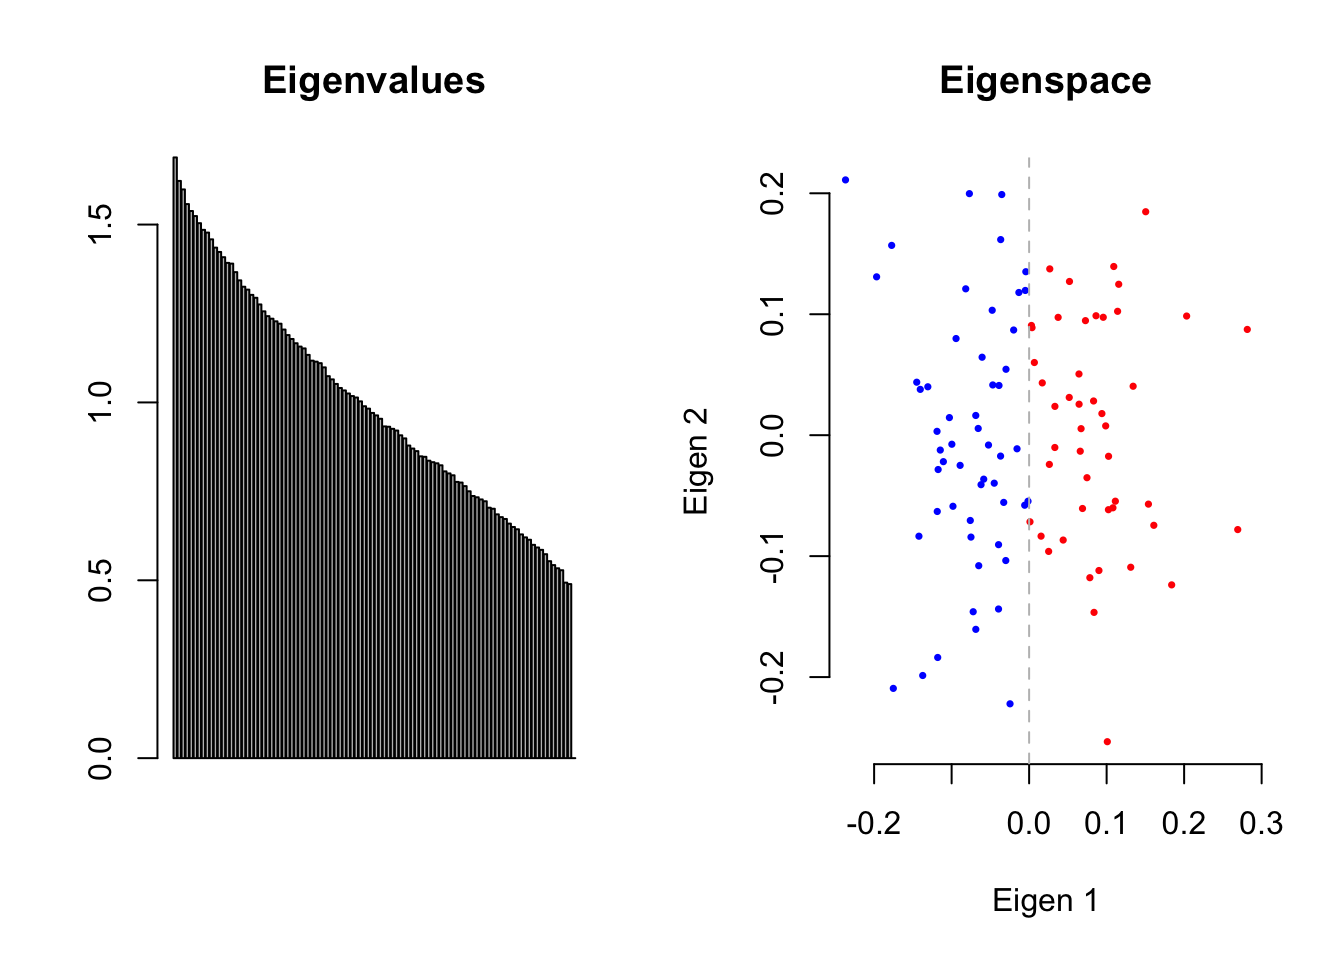
\includegraphics{EigenGWAS_files/figure-latex/eigen-1.pdf}

\hypertarget{population-structure-lambda_gc}{%
\subsection{\texorpdfstring{Population structure
\(\lambda_{GC}\)}{Population structure \textbackslash{}lambda\_\{GC\}}}\label{population-structure-lambda_gc}}

We can define \(\lambda_{GC}=\chi^2_{1,median(p)}/\chi^2_{1,0.5}\), in
which \(\chi^2_{1,0.5}=0.455\). We further use subscript \(k\) to denote
\(\lambda_{GC_k}\) the one that is estimated from \(\mathbf{E}_k\).

When the population structure is completely driven by genetic drift,
\(\lambda_{GC_k} \approx \Lambda_k\).

After technical correction, correspondingly
\(\tilde\chi^2_1=\chi^2_1/\lambda_{GC}\), a reduce of the test statistic
compared to its original form.

\begin{Shaded}
\begin{Highlighting}[]
\NormalTok{Chi=}\KeywordTok{rchisq}\NormalTok{(}\DecValTok{10000}\NormalTok{, }\DecValTok{1}\NormalTok{, }\DataTypeTok{ncp=}\FloatTok{0.2}\NormalTok{)}
\KeywordTok{layout}\NormalTok{(}\KeywordTok{matrix}\NormalTok{(}\DecValTok{1}\OperatorTok{:}\DecValTok{2}\NormalTok{, }\DecValTok{1}\NormalTok{, }\DecValTok{2}\NormalTok{))}
\KeywordTok{qqplot}\NormalTok{(}\DataTypeTok{main=}\StringTok{"Raw"}\NormalTok{, }\KeywordTok{rchisq}\NormalTok{(}\DecValTok{1000}\NormalTok{,}\DecValTok{1}\NormalTok{), Chi, }\DataTypeTok{bty=}\StringTok{"n"}\NormalTok{, }\DataTypeTok{xlab=}\KeywordTok{expression}\NormalTok{(}\KeywordTok{paste}\NormalTok{(}\StringTok{"Theoretical "}\NormalTok{,chi[}\DecValTok{1}\NormalTok{]}\OperatorTok{^}\DecValTok{2}\NormalTok{)), }\DataTypeTok{ylab=}\KeywordTok{expression}\NormalTok{(}\KeywordTok{paste}\NormalTok{(}\StringTok{"Observed "}\NormalTok{,chi[}\DecValTok{1}\NormalTok{]}\OperatorTok{^}\DecValTok{2}\NormalTok{)), }\DataTypeTok{pch=}\DecValTok{16}\NormalTok{, }\DataTypeTok{cex=}\FloatTok{0.5}\NormalTok{)}
\KeywordTok{abline}\NormalTok{(}\DataTypeTok{a=}\DecValTok{0}\NormalTok{, }\DataTypeTok{b=}\DecValTok{1}\NormalTok{, }\DataTypeTok{col=}\StringTok{"red"}\NormalTok{, }\DataTypeTok{lty=}\DecValTok{2}\NormalTok{)}
\NormalTok{gc=}\KeywordTok{median}\NormalTok{(Chi)}\OperatorTok{/}\KeywordTok{qchisq}\NormalTok{(}\FloatTok{0.5}\NormalTok{, }\DecValTok{1}\NormalTok{, }\DataTypeTok{lower.tail =}\NormalTok{ F)}
\NormalTok{ChiGC=Chi}\OperatorTok{/}\NormalTok{gc}
\KeywordTok{qqplot}\NormalTok{(}\DataTypeTok{main=}\StringTok{"After correction"}\NormalTok{, }\KeywordTok{rchisq}\NormalTok{(}\DecValTok{1000}\NormalTok{,}\DecValTok{1}\NormalTok{), ChiGC, }\DataTypeTok{bty=}\StringTok{"n"}\NormalTok{, }\DataTypeTok{xlab=}\KeywordTok{expression}\NormalTok{(}\KeywordTok{paste}\NormalTok{(}\StringTok{"Theoretical "}\NormalTok{,chi[}\DecValTok{1}\NormalTok{]}\OperatorTok{^}\DecValTok{2}\NormalTok{)), }\DataTypeTok{ylab=}\KeywordTok{expression}\NormalTok{(}\KeywordTok{paste}\NormalTok{(}\StringTok{"Observed "}\NormalTok{,chi[}\DecValTok{1}\NormalTok{]}\OperatorTok{^}\DecValTok{2}\NormalTok{)), }\DataTypeTok{pch=}\DecValTok{16}\NormalTok{, }\DataTypeTok{cex=}\FloatTok{0.5}\NormalTok{)}
\KeywordTok{abline}\NormalTok{(}\DataTypeTok{a=}\DecValTok{0}\NormalTok{, }\DataTypeTok{b=}\DecValTok{1}\NormalTok{, }\DataTypeTok{col=}\StringTok{"red"}\NormalTok{, }\DataTypeTok{lty=}\DecValTok{2}\NormalTok{)}
\end{Highlighting}
\end{Shaded}

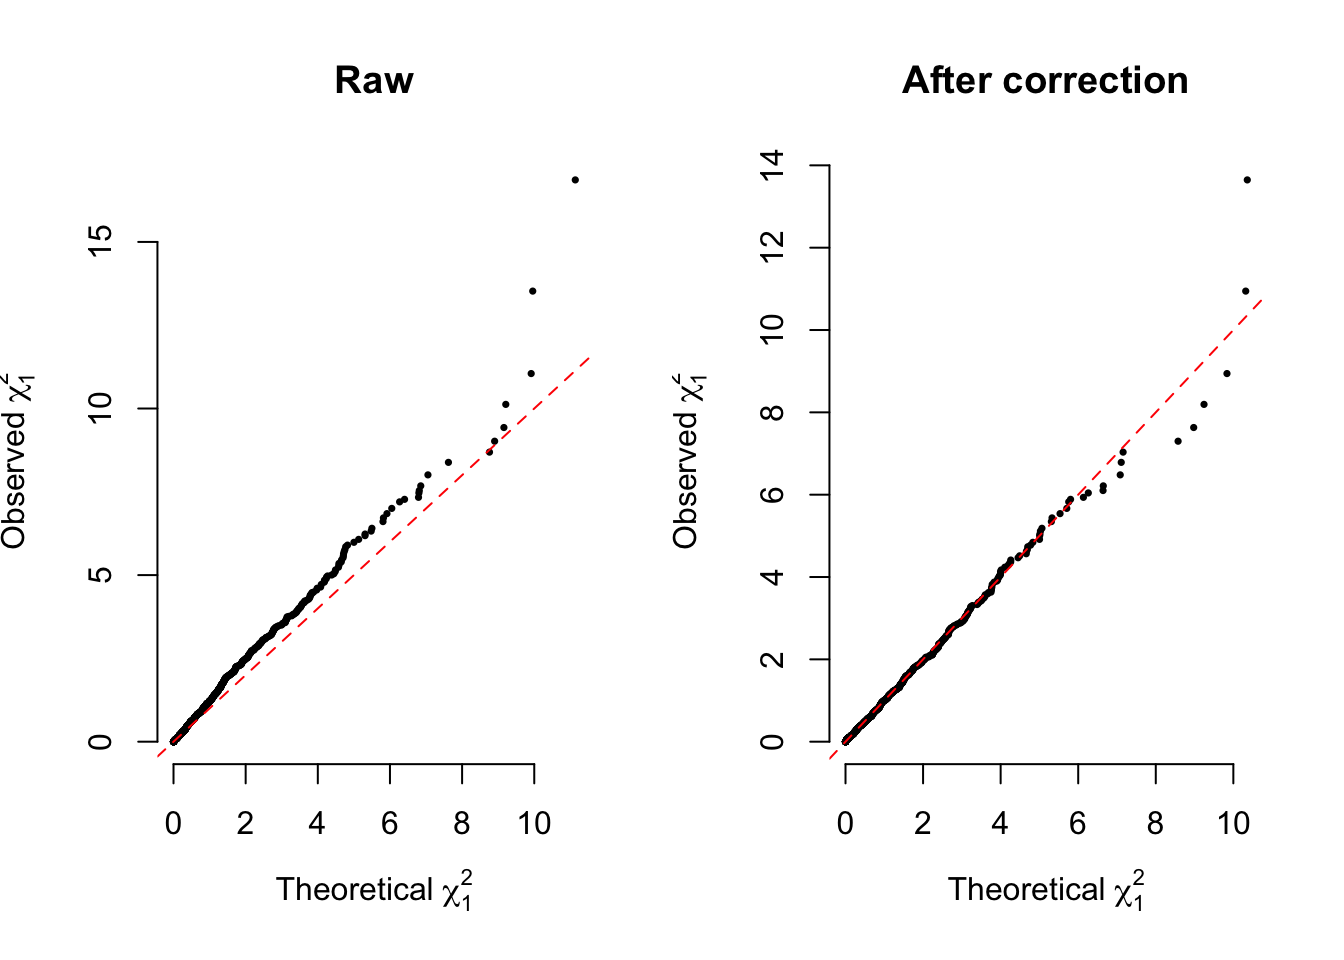
\includegraphics{EigenGWAS_files/figure-latex/gc-1.pdf}

\hypertarget{threshold-for-eigengwas}{%
\subsection{Threshold for EigenGWAS}\label{threshold-for-eigengwas}}

As shown above, EigenGWAS Bonferroni correction, such as \(\alpha/m\),
can be used to set the threshold at the significance level \(\alpha\),
such as \(\alpha=0.05\).

\hypertarget{connection-to-svd}{%
\section{Connection to SVD}\label{connection-to-svd}}

SVD of \(\mathbf{X}=\mathbf{U\Lambda V}\), the EigenGWAS model can be
written as \(\mathbf{V}_k=\frac{\mathbf{XU}_k}{\Lambda_k}\). However, in
this transformation, eigenvalue is involved, as would be show. It will
reduce the statistical power for EigenGWAS.

\hypertarget{intepretation}{%
\section{Intepretation}\label{intepretation}}

The EigenGWAS model resembles the Newtown's first and the second law for
classical mechanics. The first law states that

\begin{quote}
In an inertial frame of reference, an object either remains at rest or
continues to move at a constant velocity, unless acted upon by a force.
\end{quote}

Analogously, in population genetics, it can be seemed as genetic drift
that is constantly driving the a pair of population apart from each
other, and its velocity can be quantified by a binomial distribution as
\(\frac{pq}{\tilde{n}_e}\).

\begin{quote}
In an inertial frame of reference, the vector sum of the forces \(F\) on
an object is equal to the mass m of that object multiplied by the
acceleration a of the object: \(F = ma\).
\end{quote}

Analogously, the selection can drive a genomic region run against its
reference population at a velocity greater than
\(\frac{pq}{\tilde{n}_e}\).

\hypertarget{protocol}{%
\chapter{Protocol}\label{protocol}}

\hypertarget{protocols-for-selection}{%
\section{Protocols for selection}\label{protocols-for-selection}}

\begin{enumerate}
\def\labelenumi{\arabic{enumi}.}
\item
  Constructing genetic relationship matrix \(\mathbf{G}\). The
  difference between a random mating population and inbred population is
  the way \(\mathbf{G}\) is constructed. So for a pair of individuals
  \(i\) and \(j\),
  \[G_{ij}=\frac{1}{\tilde{m}}\sum_l^{\tilde{m}}\frac{(x_{il}-2p_l)(x_{jl}-2p_l)}{2(1+F)p_iq_i}\]
  and \(F=1\) for inbred lines.
\item
  Conducting eigenanalysis for \(\mathbf{G}\).
\item
  Linear regression analysis for each SNP.
\end{enumerate}

\hypertarget{rscript-pipeline-for-random-mating-population}{%
\subsection{Rscript pipeline for random mating
population}\label{rscript-pipeline-for-random-mating-population}}

\begin{Shaded}
\begin{Highlighting}[]
\NormalTok{plink2=}\StringTok{'/Users/gc5k/bin/plink_mac/plink'}
\NormalTok{dat=}\StringTok{"./data/euro/euro"}

\CommentTok{#make-grm}
\NormalTok{grmCmd=}\KeywordTok{paste}\NormalTok{(plink2, }\StringTok{"--bfile "}\NormalTok{, dat, }\StringTok{"--make-grm-gz --out "}\NormalTok{, dat)}
\KeywordTok{system}\NormalTok{(grmCmd)}

\NormalTok{gz=}\KeywordTok{gzfile}\NormalTok{(}\KeywordTok{paste0}\NormalTok{(dat, }\StringTok{".grm.gz"}\NormalTok{))}
\NormalTok{grm=}\KeywordTok{read.table}\NormalTok{(gz, }\DataTypeTok{as.is =}\NormalTok{ T)}
\NormalTok{Ne=}\OperatorTok{-}\DecValTok{1}\OperatorTok{/}\KeywordTok{mean}\NormalTok{(grm[grm[,}\DecValTok{1}\NormalTok{]}\OperatorTok{!=}\NormalTok{grm[,}\DecValTok{2}\NormalTok{], }\DecValTok{4}\NormalTok{])}
\NormalTok{Me=}\DecValTok{1}\OperatorTok{/}\KeywordTok{var}\NormalTok{(grm[grm[,}\DecValTok{1}\NormalTok{]}\OperatorTok{!=}\NormalTok{grm[,}\DecValTok{2}\NormalTok{], }\DecValTok{4}\NormalTok{])}
\KeywordTok{print}\NormalTok{(}\KeywordTok{paste}\NormalTok{(}\StringTok{"Ne="}\NormalTok{, }\KeywordTok{format}\NormalTok{(Ne, }\DataTypeTok{digits =} \DecValTok{2}\NormalTok{), }\StringTok{"Me="}\NormalTok{, }\KeywordTok{format}\NormalTok{(Me, }\DataTypeTok{digits =} \DecValTok{2}\NormalTok{)))}
\CommentTok{## [1] "Ne= 199 Me= 21870"}

\CommentTok{#pca}
\NormalTok{pcaCmd=}\KeywordTok{paste}\NormalTok{(plink2, }\StringTok{"--bfile "}\NormalTok{, dat, }\StringTok{"--pca 5 --out "}\NormalTok{, dat)}
\KeywordTok{system}\NormalTok{(pcaCmd)}
\KeywordTok{barplot}\NormalTok{(}\KeywordTok{read.table}\NormalTok{(}\KeywordTok{paste0}\NormalTok{(dat, }\StringTok{".eigenval"}\NormalTok{), }\DataTypeTok{as.is =}\NormalTok{ T)[,}\DecValTok{1}\NormalTok{]}\OperatorTok{/}\DecValTok{2}\NormalTok{, }\DataTypeTok{border =}\NormalTok{ F)}
\end{Highlighting}
\end{Shaded}

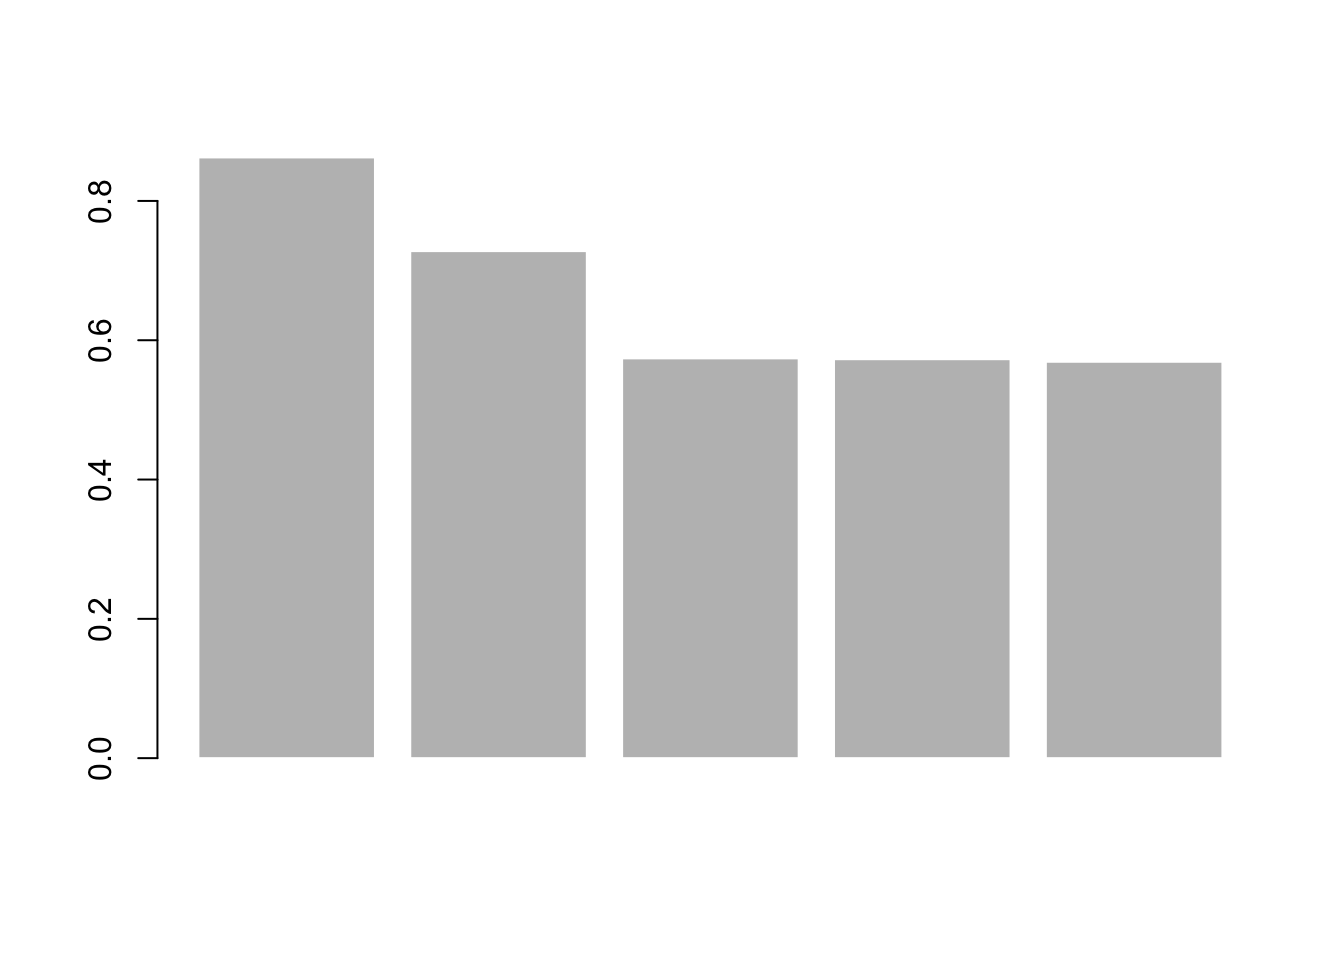
\includegraphics{EigenGWAS_files/figure-latex/euro-demo-1.pdf}

\begin{Shaded}
\begin{Highlighting}[]

\NormalTok{pc=}\KeywordTok{read.table}\NormalTok{(}\KeywordTok{paste0}\NormalTok{(dat, }\StringTok{".eigenvec"}\NormalTok{), }\DataTypeTok{as.is =}\NormalTok{ T)}
\KeywordTok{plot}\NormalTok{(pc[,}\DecValTok{3}\NormalTok{], pc[,}\DecValTok{4}\NormalTok{], }\DataTypeTok{xlab=}\StringTok{"Eigenvector 1"}\NormalTok{, }\DataTypeTok{ylab=}\StringTok{"Eigenvector 2"}\NormalTok{, }\DataTypeTok{bty=}\StringTok{"n"}\NormalTok{, }\DataTypeTok{main=}\StringTok{"Eigenspace"}\NormalTok{, }\DataTypeTok{bty=}\StringTok{"n"}\NormalTok{, }\DataTypeTok{col=}\KeywordTok{ifelse}\NormalTok{(pc[,}\DecValTok{3}\NormalTok{]}\OperatorTok{>}\DecValTok{0}\NormalTok{, }\StringTok{"red"}\NormalTok{, }\StringTok{"blue"}\NormalTok{), }\DataTypeTok{pch=}\DecValTok{16}\NormalTok{, }\DataTypeTok{cex=}\FloatTok{0.5}\NormalTok{)}
\end{Highlighting}
\end{Shaded}

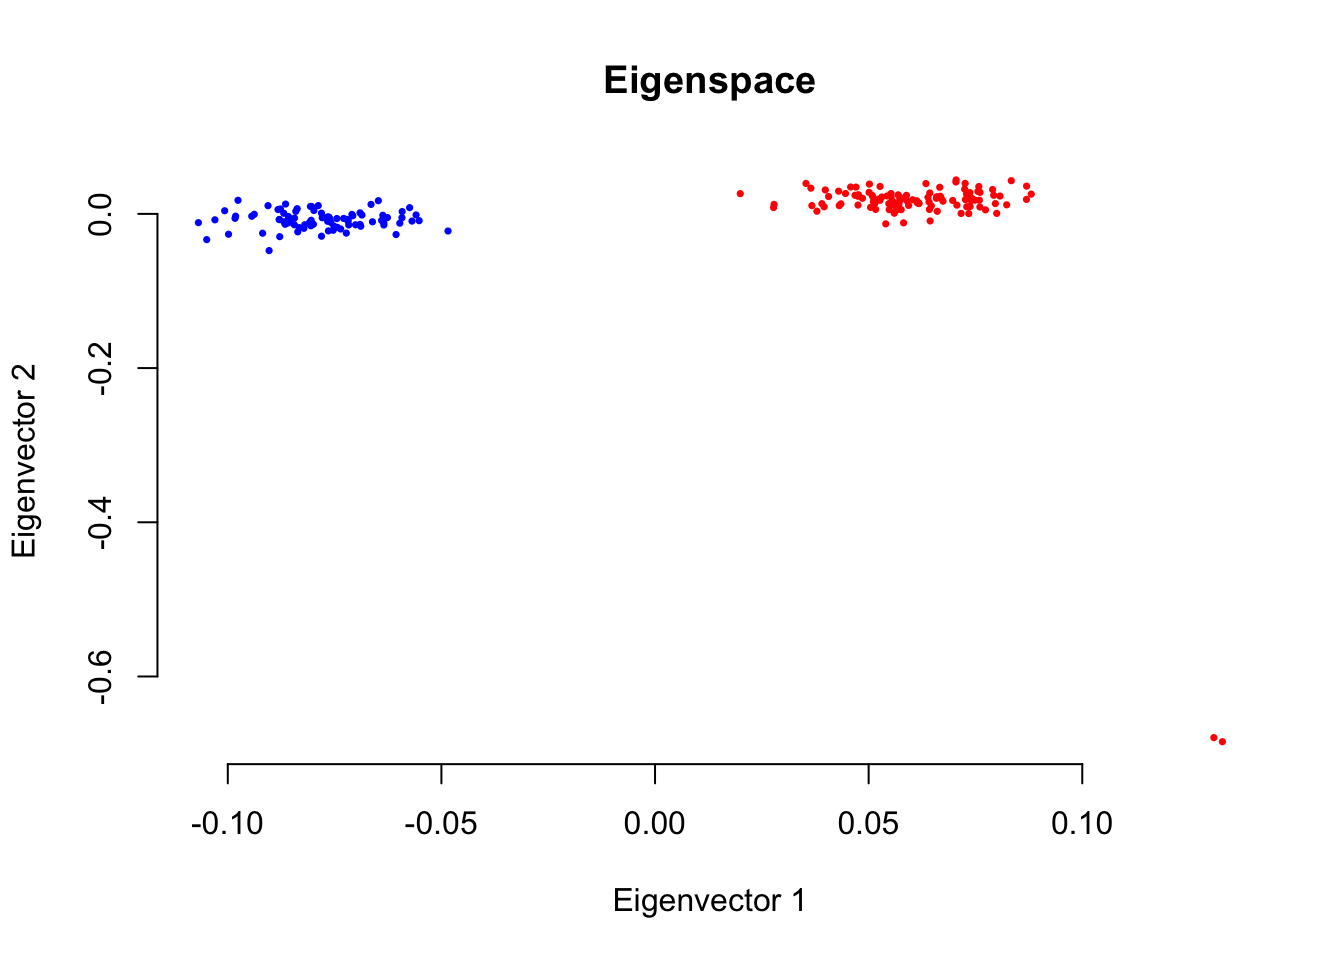
\includegraphics{EigenGWAS_files/figure-latex/euro-demo-2.pdf}

\begin{Shaded}
\begin{Highlighting}[]
\CommentTok{#make-grm}
\KeywordTok{source}\NormalTok{(}\StringTok{"~/R/MyLib/manhattan.R"}\NormalTok{)}
\NormalTok{liCmd=}\KeywordTok{paste0}\NormalTok{(plink2, }\StringTok{" --linear --bfile "}\NormalTok{, dat, }\StringTok{" --pheno "}\NormalTok{, dat, }\StringTok{".eigenvec --out "}\NormalTok{, dat)}
\KeywordTok{system}\NormalTok{(liCmd)}

\CommentTok{#plot}
\NormalTok{EigenRes=}\KeywordTok{read.table}\NormalTok{(}\KeywordTok{paste0}\NormalTok{(dat, }\StringTok{".assoc.linear"}\NormalTok{), }\DataTypeTok{as.is =}\NormalTok{ T, }\DataTypeTok{header =}\NormalTok{ T)}
\NormalTok{EigenRes}\OperatorTok{$}\NormalTok{Praw=EigenRes}\OperatorTok{$}\NormalTok{P}
\NormalTok{gc=}\KeywordTok{qchisq}\NormalTok{(}\KeywordTok{median}\NormalTok{(EigenRes}\OperatorTok{$}\NormalTok{P), }\DecValTok{1}\NormalTok{, }\DataTypeTok{lower.tail =}\NormalTok{ F)}\OperatorTok{/}\KeywordTok{qchisq}\NormalTok{(}\FloatTok{0.5}\NormalTok{, }\DecValTok{1}\NormalTok{, }\DataTypeTok{lower.tail =}\NormalTok{ F)}
\KeywordTok{print}\NormalTok{(}\KeywordTok{paste}\NormalTok{(}\StringTok{"GC = "}\NormalTok{, }\KeywordTok{format}\NormalTok{(gc, }\DataTypeTok{digits =} \DecValTok{4}\NormalTok{)))}
\CommentTok{## [1] "GC =  1.692"}
\NormalTok{EigenRes}\OperatorTok{$}\NormalTok{P=}\KeywordTok{pchisq}\NormalTok{(}\KeywordTok{qchisq}\NormalTok{(EigenRes}\OperatorTok{$}\NormalTok{Praw, }\DecValTok{1}\NormalTok{, }\DataTypeTok{lower.tail =}\NormalTok{ F)}\OperatorTok{/}\NormalTok{gc, }\DecValTok{1}\NormalTok{, }\DataTypeTok{lower.tail =}\NormalTok{ F)}
\KeywordTok{manhattan}\NormalTok{(EigenRes, }\DataTypeTok{title=}\StringTok{"EigenGWAS 1"}\NormalTok{, }\DataTypeTok{pch=}\DecValTok{16}\NormalTok{, }\DataTypeTok{cex=}\FloatTok{0.3}\NormalTok{, }\DataTypeTok{bty=}\StringTok{'n'}\NormalTok{)}
\end{Highlighting}
\end{Shaded}

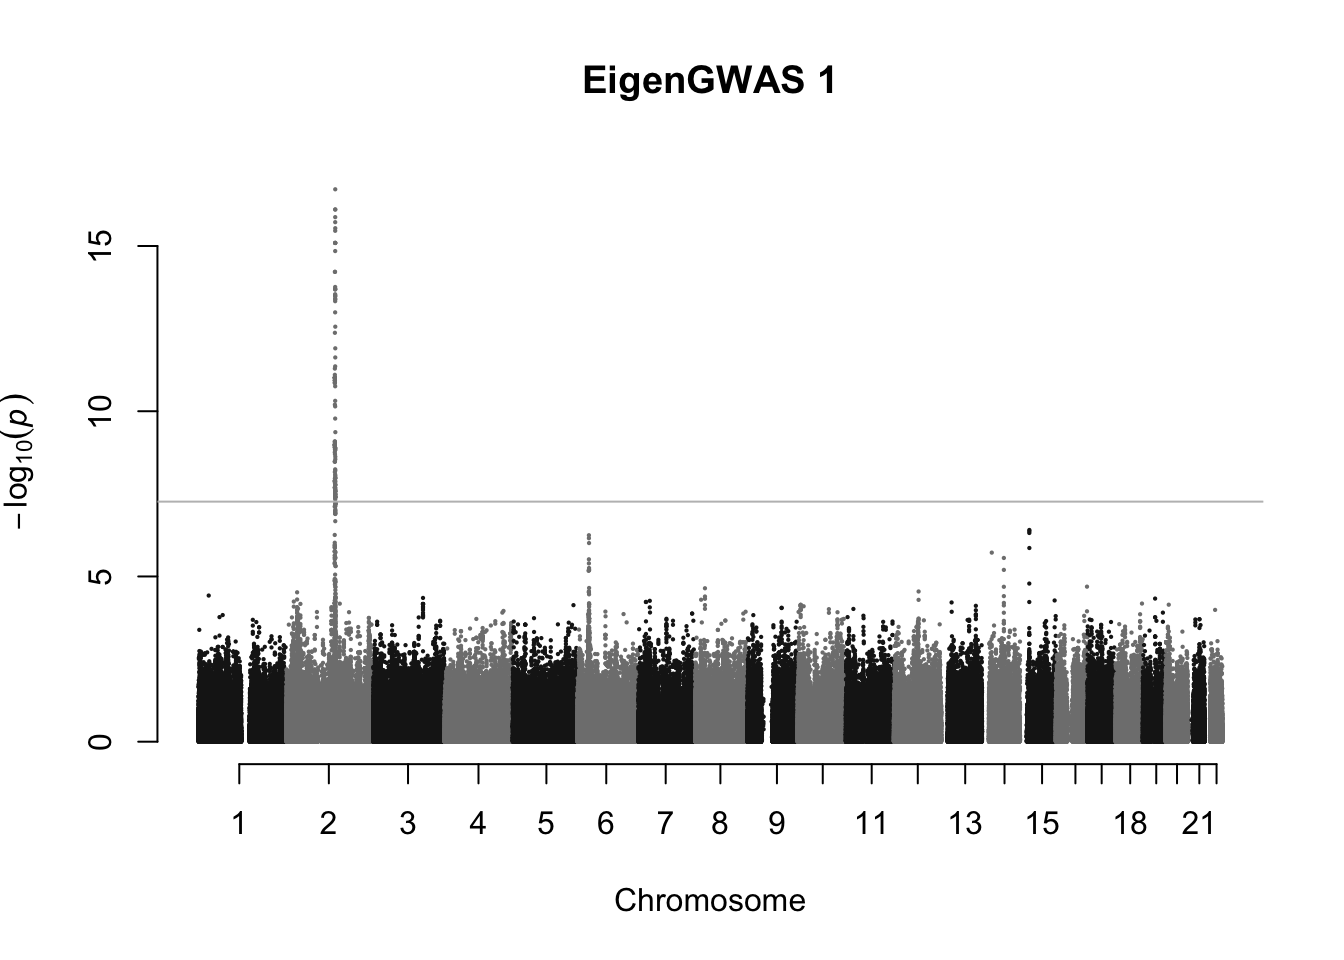
\includegraphics{EigenGWAS_files/figure-latex/euro-demo-3.pdf}

\begin{Shaded}
\begin{Highlighting}[]

\CommentTok{#QQplot}
\NormalTok{chiseq=}\KeywordTok{rchisq}\NormalTok{(}\KeywordTok{nrow}\NormalTok{(EigenRes), }\DecValTok{1}\NormalTok{)}
\KeywordTok{qqplot}\NormalTok{(chiseq, }\KeywordTok{qchisq}\NormalTok{(EigenRes}\OperatorTok{$}\NormalTok{Praw, }\DecValTok{1}\NormalTok{, }\DataTypeTok{lower.tail =}\NormalTok{ F), }\DataTypeTok{xlab=}\KeywordTok{expression}\NormalTok{(}\KeywordTok{paste}\NormalTok{(}\StringTok{"Theoretical "}\NormalTok{, chi[}\DecValTok{1}\NormalTok{]}\OperatorTok{^}\DecValTok{2}\NormalTok{)), }\DataTypeTok{ylab=}\KeywordTok{expression}\NormalTok{(}\KeywordTok{paste}\NormalTok{(}\StringTok{"Observed "}\NormalTok{, chi[}\DecValTok{1}\NormalTok{]}\OperatorTok{^}\DecValTok{2}\NormalTok{)), }\DataTypeTok{bty=}\StringTok{"n"}\NormalTok{, }\DataTypeTok{col=}\StringTok{"grey"}\NormalTok{, }\DataTypeTok{pch=}\DecValTok{16}\NormalTok{, }\DataTypeTok{cex=}\FloatTok{0.5}\NormalTok{)}
\KeywordTok{points}\NormalTok{(}\KeywordTok{sort}\NormalTok{(chiseq), }\KeywordTok{sort}\NormalTok{(}\KeywordTok{qchisq}\NormalTok{(EigenRes}\OperatorTok{$}\NormalTok{P, }\DecValTok{1}\NormalTok{, }\DataTypeTok{lower.tail =}\NormalTok{ F)), }\DataTypeTok{col=}\StringTok{"black"}\NormalTok{, }\DataTypeTok{pch=}\DecValTok{16}\NormalTok{, }\DataTypeTok{cex=}\FloatTok{0.5}\NormalTok{)}
\KeywordTok{legend}\NormalTok{(}\StringTok{"topleft"}\NormalTok{, }\DataTypeTok{legend =} \KeywordTok{c}\NormalTok{(}\StringTok{"Raw"}\NormalTok{, }\StringTok{"GC correction"}\NormalTok{), }\DataTypeTok{pch=}\DecValTok{16}\NormalTok{, }\DataTypeTok{cex=}\FloatTok{0.5}\NormalTok{, }\DataTypeTok{col=}\KeywordTok{c}\NormalTok{(}\StringTok{"grey"}\NormalTok{, }\StringTok{"black"}\NormalTok{), }\DataTypeTok{bty=}\StringTok{'n'}\NormalTok{)}
\KeywordTok{abline}\NormalTok{(}\DataTypeTok{a=}\DecValTok{0}\NormalTok{, }\DataTypeTok{b=}\DecValTok{1}\NormalTok{, }\DataTypeTok{col=}\StringTok{"red"}\NormalTok{, }\DataTypeTok{lty=}\DecValTok{2}\NormalTok{)}
\end{Highlighting}
\end{Shaded}

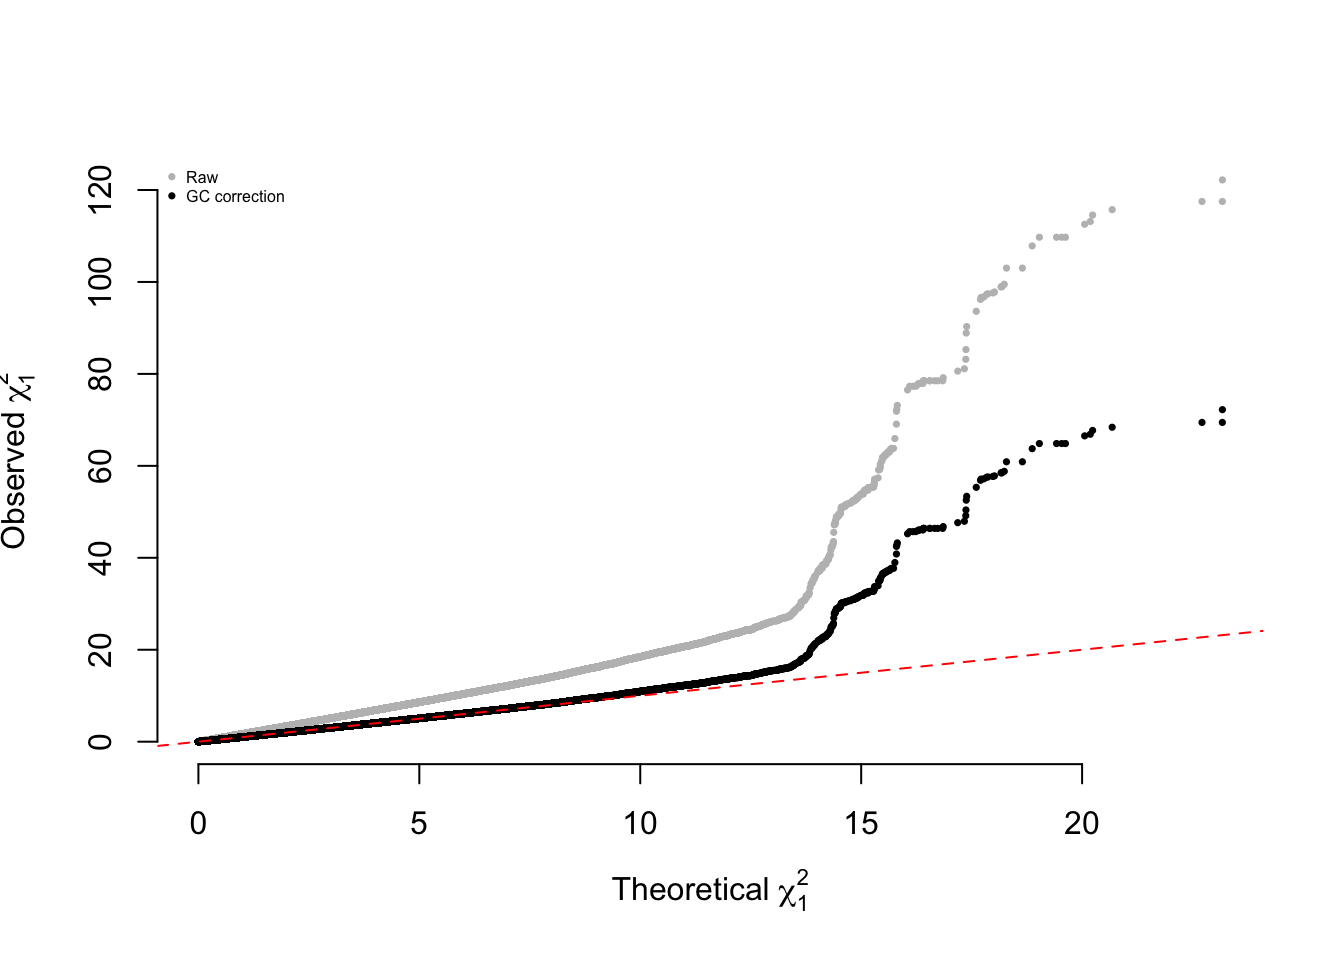
\includegraphics{EigenGWAS_files/figure-latex/euro-demo-4.pdf}

\hypertarget{rscript-pipeline-for-inbred-population}{%
\subsection{Rscript pipeline for inbred
population}\label{rscript-pipeline-for-inbred-population}}

\begin{Shaded}
\begin{Highlighting}[]
\NormalTok{plink2=}\StringTok{'/Users/gc5k/bin/plink_mac/plink'}
\NormalTok{dat=}\StringTok{"./data/arab/arab"}

\CommentTok{#make-grm}
\NormalTok{grmCmd=}\KeywordTok{paste}\NormalTok{(plink2, }\StringTok{"--bfile "}\NormalTok{, dat, }\StringTok{"--make-grm-gz --out "}\NormalTok{, dat)}
\KeywordTok{system}\NormalTok{(grmCmd)}

\NormalTok{gz=}\KeywordTok{gzfile}\NormalTok{(}\KeywordTok{paste0}\NormalTok{(dat, }\StringTok{".grm.gz"}\NormalTok{))}
\NormalTok{grm=}\KeywordTok{read.table}\NormalTok{(gz, }\DataTypeTok{as.is =}\NormalTok{ T)}
\NormalTok{Ne=}\OperatorTok{-}\DecValTok{1}\OperatorTok{/}\KeywordTok{mean}\NormalTok{(grm[grm[,}\DecValTok{1}\NormalTok{]}\OperatorTok{!=}\NormalTok{grm[,}\DecValTok{2}\NormalTok{], }\DecValTok{4}\NormalTok{]}\OperatorTok{/}\DecValTok{2}\NormalTok{)}
\NormalTok{Me=}\DecValTok{1}\OperatorTok{/}\KeywordTok{var}\NormalTok{(grm[grm[,}\DecValTok{1}\NormalTok{]}\OperatorTok{!=}\NormalTok{grm[,}\DecValTok{2}\NormalTok{], }\DecValTok{4}\NormalTok{]}\OperatorTok{/}\DecValTok{2}\NormalTok{)}
\KeywordTok{print}\NormalTok{(}\KeywordTok{paste}\NormalTok{(}\StringTok{"Ne="}\NormalTok{, }\KeywordTok{format}\NormalTok{(Ne, }\DataTypeTok{digits =} \DecValTok{2}\NormalTok{), }\StringTok{"Me="}\NormalTok{, }\KeywordTok{format}\NormalTok{(Me, }\DataTypeTok{digits =} \DecValTok{2}\NormalTok{)))}
\CommentTok{## [1] "Ne= 293 Me= 395"}

\CommentTok{#pca}
\NormalTok{pcaCmd=}\KeywordTok{paste}\NormalTok{(plink2, }\StringTok{"--bfile "}\NormalTok{, dat, }\StringTok{"--pca 5 --out "}\NormalTok{, dat)}
\KeywordTok{system}\NormalTok{(pcaCmd)}
\KeywordTok{barplot}\NormalTok{(}\KeywordTok{read.table}\NormalTok{(}\KeywordTok{paste0}\NormalTok{(dat, }\StringTok{".eigenval"}\NormalTok{), }\DataTypeTok{as.is =}\NormalTok{ T)[,}\DecValTok{1}\NormalTok{]}\OperatorTok{/}\DecValTok{2}\NormalTok{, }\DataTypeTok{border =}\NormalTok{ F)}
\end{Highlighting}
\end{Shaded}

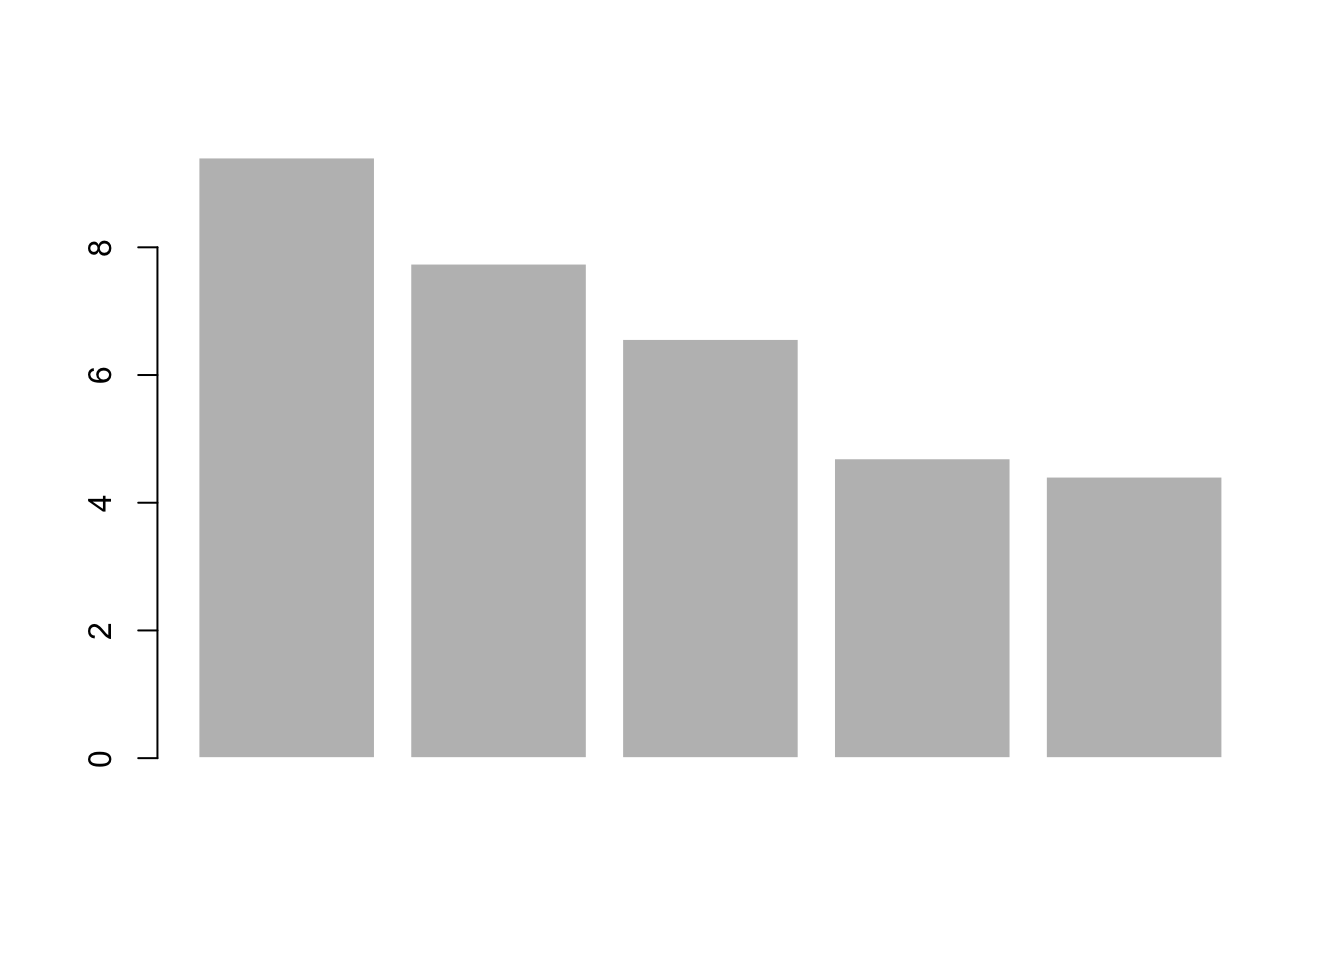
\includegraphics{EigenGWAS_files/figure-latex/arab-demo-1.pdf}

\begin{Shaded}
\begin{Highlighting}[]

\NormalTok{pc=}\KeywordTok{read.table}\NormalTok{(}\KeywordTok{paste0}\NormalTok{(dat, }\StringTok{".eigenvec"}\NormalTok{), }\DataTypeTok{as.is =}\NormalTok{ T)}
\KeywordTok{plot}\NormalTok{(pc[,}\DecValTok{3}\NormalTok{], pc[,}\DecValTok{4}\NormalTok{], }\DataTypeTok{xlab=}\StringTok{"Eigenvector 1"}\NormalTok{, }\DataTypeTok{ylab=}\StringTok{"Eigenvector 2"}\NormalTok{, }\DataTypeTok{bty=}\StringTok{"n"}\NormalTok{, }\DataTypeTok{main=}\StringTok{"Eigenspace"}\NormalTok{, }\DataTypeTok{bty=}\StringTok{"n"}\NormalTok{, }\DataTypeTok{col=}\KeywordTok{ifelse}\NormalTok{(pc[,}\DecValTok{3}\NormalTok{]}\OperatorTok{>}\DecValTok{0}\NormalTok{, }\StringTok{"red"}\NormalTok{, }\StringTok{"blue"}\NormalTok{), }\DataTypeTok{pch=}\DecValTok{16}\NormalTok{, }\DataTypeTok{cex=}\FloatTok{0.5}\NormalTok{)}
\end{Highlighting}
\end{Shaded}

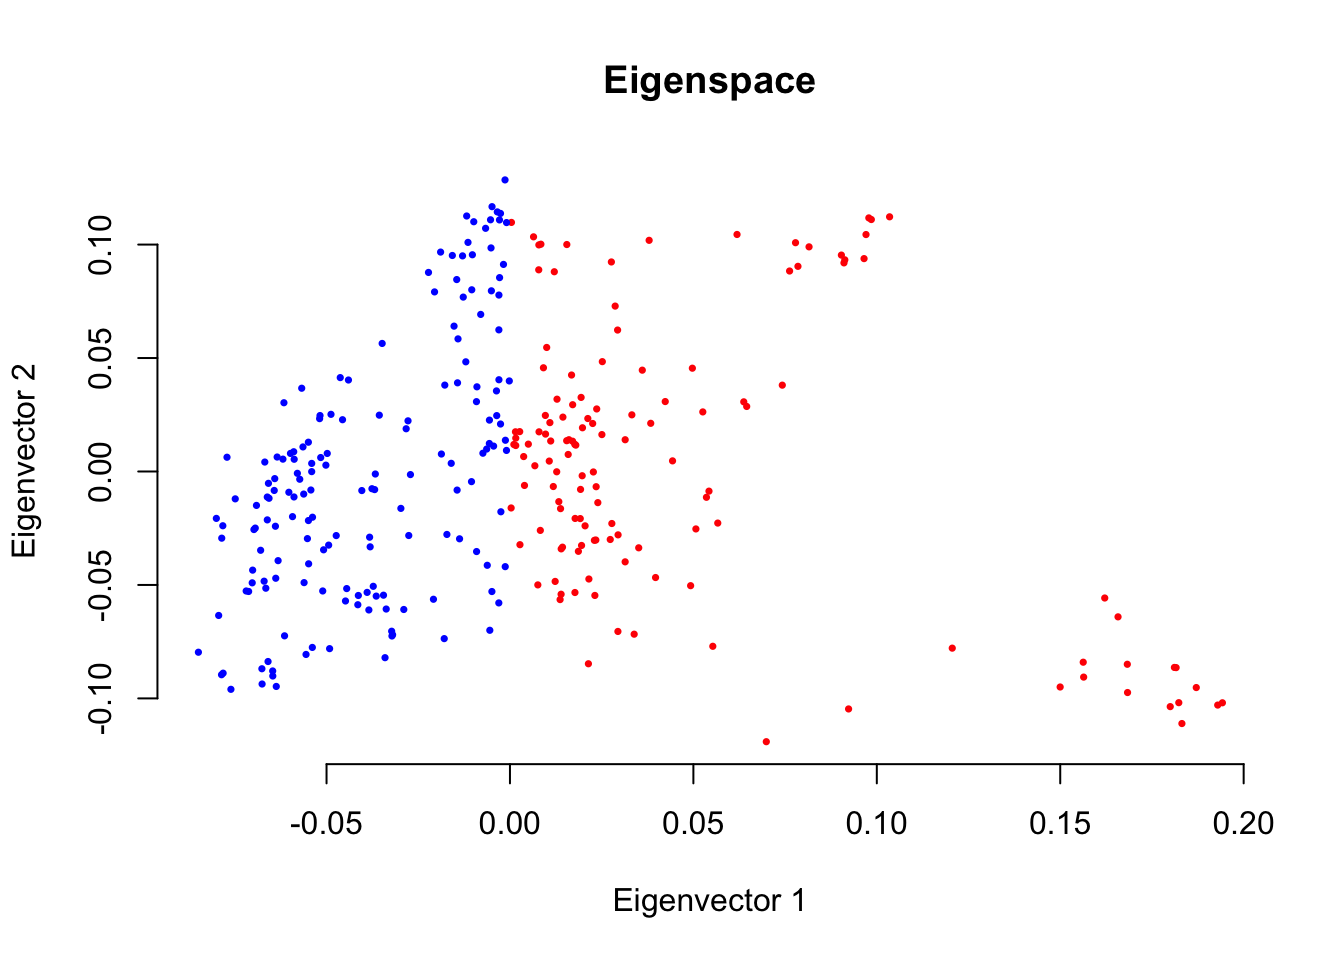
\includegraphics{EigenGWAS_files/figure-latex/arab-demo-2.pdf}

\begin{Shaded}
\begin{Highlighting}[]
\CommentTok{#make-grm}
\KeywordTok{source}\NormalTok{(}\StringTok{"~/R/MyLib/manhattan.R"}\NormalTok{)}
\NormalTok{liCmd=}\KeywordTok{paste0}\NormalTok{(plink2, }\StringTok{" --linear --bfile "}\NormalTok{, dat, }\StringTok{" --pheno "}\NormalTok{, dat, }\StringTok{".eigenvec --out "}\NormalTok{, dat)}
\KeywordTok{system}\NormalTok{(liCmd)}

\CommentTok{#plot}
\NormalTok{EigenRes=}\KeywordTok{read.table}\NormalTok{(}\KeywordTok{paste0}\NormalTok{(dat, }\StringTok{".assoc.linear"}\NormalTok{), }\DataTypeTok{as.is =}\NormalTok{ T, }\DataTypeTok{header =}\NormalTok{ T)}
\NormalTok{EigenRes}\OperatorTok{$}\NormalTok{Praw=EigenRes}\OperatorTok{$}\NormalTok{P}
\NormalTok{gc=}\KeywordTok{qchisq}\NormalTok{(}\KeywordTok{median}\NormalTok{(EigenRes}\OperatorTok{$}\NormalTok{P), }\DecValTok{1}\NormalTok{, }\DataTypeTok{lower.tail =}\NormalTok{ F)}\OperatorTok{/}\KeywordTok{qchisq}\NormalTok{(}\FloatTok{0.5}\NormalTok{, }\DecValTok{1}\NormalTok{, }\DataTypeTok{lower.tail =}\NormalTok{ F)}
\KeywordTok{print}\NormalTok{(}\KeywordTok{paste}\NormalTok{(}\StringTok{"GC = "}\NormalTok{, }\KeywordTok{format}\NormalTok{(gc, }\DataTypeTok{digits =} \DecValTok{4}\NormalTok{)))}
\CommentTok{## [1] "GC =  9.047"}
\NormalTok{EigenRes}\OperatorTok{$}\NormalTok{P=}\KeywordTok{pchisq}\NormalTok{(}\KeywordTok{qchisq}\NormalTok{(EigenRes}\OperatorTok{$}\NormalTok{Praw, }\DecValTok{1}\NormalTok{, }\DataTypeTok{lower.tail =}\NormalTok{ F)}\OperatorTok{/}\NormalTok{gc, }\DecValTok{1}\NormalTok{, }\DataTypeTok{lower.tail =}\NormalTok{ F)}
\KeywordTok{manhattan}\NormalTok{(EigenRes, }\DataTypeTok{title=}\StringTok{"EigenGWAS 1"}\NormalTok{, }\DataTypeTok{pch=}\DecValTok{16}\NormalTok{, }\DataTypeTok{cex=}\FloatTok{0.3}\NormalTok{, }\DataTypeTok{bty=}\StringTok{'n'}\NormalTok{)}
\end{Highlighting}
\end{Shaded}

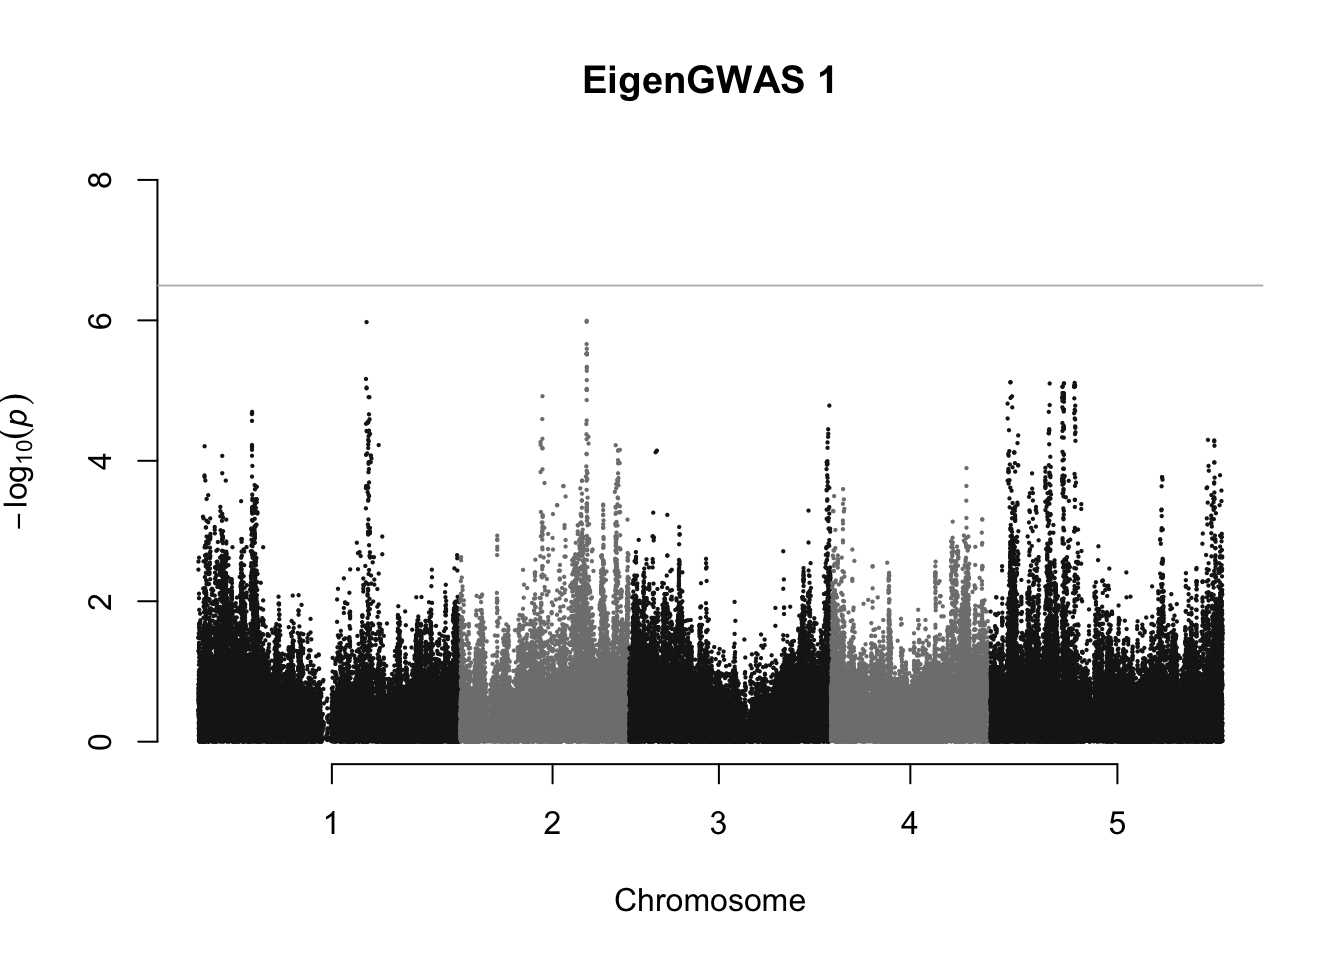
\includegraphics{EigenGWAS_files/figure-latex/arab-demo-3.pdf}

\begin{Shaded}
\begin{Highlighting}[]

\CommentTok{#QQplot}
\NormalTok{chiseq=}\KeywordTok{rchisq}\NormalTok{(}\KeywordTok{nrow}\NormalTok{(EigenRes), }\DecValTok{1}\NormalTok{)}
\KeywordTok{qqplot}\NormalTok{(chiseq, }\KeywordTok{qchisq}\NormalTok{(EigenRes}\OperatorTok{$}\NormalTok{Praw, }\DecValTok{1}\NormalTok{, }\DataTypeTok{lower.tail =}\NormalTok{ F), }\DataTypeTok{xlab=}\KeywordTok{expression}\NormalTok{(}\KeywordTok{paste}\NormalTok{(}\StringTok{"Theoretical "}\NormalTok{, chi[}\DecValTok{1}\NormalTok{]}\OperatorTok{^}\DecValTok{2}\NormalTok{)), }\DataTypeTok{ylab=}\KeywordTok{expression}\NormalTok{(}\KeywordTok{paste}\NormalTok{(}\StringTok{"Observed "}\NormalTok{, chi[}\DecValTok{1}\NormalTok{]}\OperatorTok{^}\DecValTok{2}\NormalTok{)), }\DataTypeTok{bty=}\StringTok{"n"}\NormalTok{, }\DataTypeTok{col=}\StringTok{"grey"}\NormalTok{, }\DataTypeTok{pch=}\DecValTok{16}\NormalTok{, }\DataTypeTok{cex=}\FloatTok{0.5}\NormalTok{)}
\KeywordTok{points}\NormalTok{(}\KeywordTok{sort}\NormalTok{(chiseq), }\KeywordTok{sort}\NormalTok{(}\KeywordTok{qchisq}\NormalTok{(EigenRes}\OperatorTok{$}\NormalTok{P, }\DecValTok{1}\NormalTok{, }\DataTypeTok{lower.tail =}\NormalTok{ F)), }\DataTypeTok{col=}\StringTok{"black"}\NormalTok{, }\DataTypeTok{pch=}\DecValTok{16}\NormalTok{, }\DataTypeTok{cex=}\FloatTok{0.5}\NormalTok{)}
\KeywordTok{legend}\NormalTok{(}\StringTok{"topleft"}\NormalTok{, }\DataTypeTok{legend =} \KeywordTok{c}\NormalTok{(}\StringTok{"Raw"}\NormalTok{, }\StringTok{"GC correction"}\NormalTok{), }\DataTypeTok{pch=}\DecValTok{16}\NormalTok{, }\DataTypeTok{cex=}\FloatTok{0.5}\NormalTok{, }\DataTypeTok{col=}\KeywordTok{c}\NormalTok{(}\StringTok{"grey"}\NormalTok{, }\StringTok{"black"}\NormalTok{), }\DataTypeTok{bty=}\StringTok{'n'}\NormalTok{)}
\KeywordTok{abline}\NormalTok{(}\DataTypeTok{a=}\DecValTok{0}\NormalTok{, }\DataTypeTok{b=}\DecValTok{1}\NormalTok{, }\DataTypeTok{col=}\StringTok{"red"}\NormalTok{, }\DataTypeTok{lty=}\DecValTok{2}\NormalTok{)}
\end{Highlighting}
\end{Shaded}

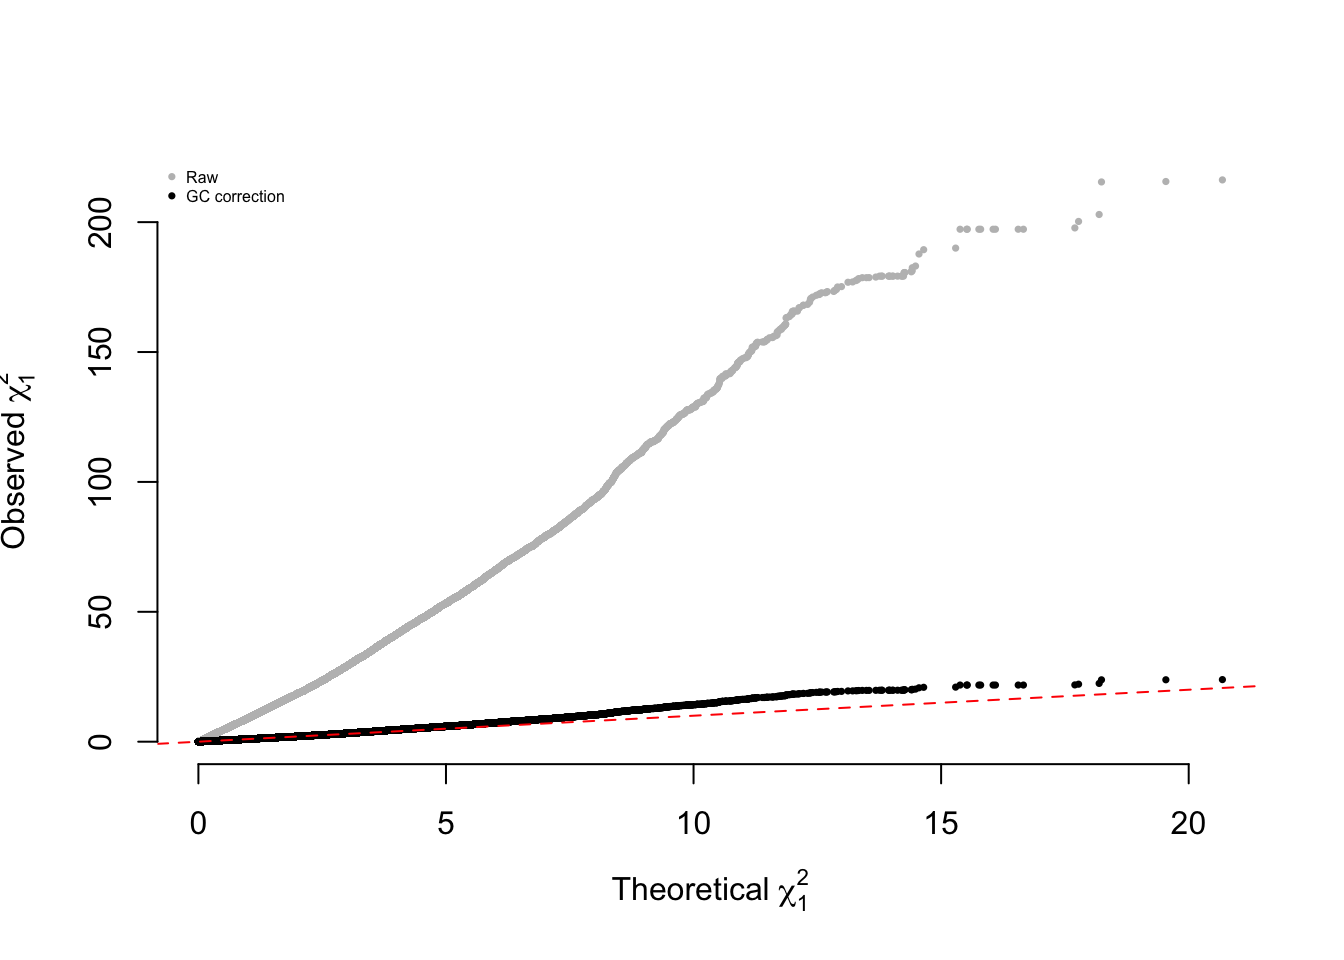
\includegraphics{EigenGWAS_files/figure-latex/arab-demo-4.pdf}

\hypertarget{protocol-for-predicted-eigenvectors}{%
\section{Protocol for predicted
eigenvectors}\label{protocol-for-predicted-eigenvectors}}

The prediction accuracy can be written as
\[R^2 \approx \frac{1}{1+\frac{n_e}{m}}\]

\hypertarget{resequencing-studies}{%
\chapter{Resequencing studies}\label{resequencing-studies}}

This is a technical review for resequencing studies.

\hypertarget{technical-review}{%
\section{Technical review}\label{technical-review}}

\hypertarget{ngs}{%
\subsection{NGS}\label{ngs}}

\hypertarget{chip-data}{%
\subsection{Chip data}\label{chip-data}}

\hypertarget{gbs}{%
\subsection{GBS}\label{gbs}}

\hypertarget{drop-hwe-test}{%
\section{Drop HWE test}\label{drop-hwe-test}}

\hypertarget{simulating-population-structure}{%
\chapter{Simulating population
structure}\label{simulating-population-structure}}

\href{http://rpubs.com/gc5k/EigenGWAScore}{Details}

\hypertarget{genetic-drift}{%
\section{Genetic drift}\label{genetic-drift}}

As each locus follows binomial distribution, the \textbf{genetic drift}
can be modelled \(\frac{\sqrt{pq}}{2n_e}\), in which \(n_e\) is the
effective population size.

\hypertarget{three-pop}{%
\section{Three pop}\label{three-pop}}

\hypertarget{six-pop}{%
\section{Six pop}\label{six-pop}}

\hypertarget{wishart-distribution-simulation}{%
\section{Wishart distribution
simulation}\label{wishart-distribution-simulation}}

\hypertarget{distribution-of-the-wishart-diagonal-elements}{%
\section{Distribution of the Wishart diagonal
elements}\label{distribution-of-the-wishart-diagonal-elements}}

\hypertarget{homo-cohort}{%
\section{Homo cohort}\label{homo-cohort}}

\hypertarget{heterogeneous-cohort}{%
\section{Heterogeneous cohort}\label{heterogeneous-cohort}}

\hypertarget{tracy-widom-distribution}{%
\section{Tracy-Widom distribution}\label{tracy-widom-distribution}}

\hypertarget{data-analysis}{%
\chapter{Data analysis}\label{data-analysis}}

\hypertarget{on-site-examples}{%
\section{On site examples}\label{on-site-examples}}

\hypertarget{arabdiopsis}{%
\subsection{Arabdiopsis}\label{arabdiopsis}}

\hypertarget{k-rice}{%
\subsection{3K rice}\label{k-rice}}

\hypertarget{als}{%
\subsection{ALS}\label{als}}

\hypertarget{gf}{%
\subsection{GF}\label{gf}}

\hypertarget{uk-birds}{%
\subsection{UK birds}\label{uk-birds}}

\hypertarget{darwins-finches}{%
\subsection{Darwin's finches}\label{darwins-finches}}

\hypertarget{gbs-maize}{%
\subsection{GBS Maize}\label{gbs-maize}}

\hypertarget{uk-biobank}{%
\subsection{UK Biobank}\label{uk-biobank}}

\hypertarget{public-datahub-neo}{%
\section{Public datahub (NEO)}\label{public-datahub-neo}}

\hypertarget{meta-research}{%
\chapter{Meta-research}\label{meta-research}}

Meta-research

\hypertarget{n_e}{%
\section{\texorpdfstring{\(n_e\)}{n\_e}}\label{n_e}}

\hypertarget{m_e}{%
\section{\texorpdfstring{\(m_e\)}{m\_e}}\label{m_e}}

\hypertarget{conclusion}{%
\chapter{Conclusion}\label{conclusion}}

\hypertarget{statistical-power}{%
\section{Statistical power}\label{statistical-power}}

\hypertarget{selection-pattern}{%
\section{Selection pattern}\label{selection-pattern}}

\bibliography{book.bib,packages.bib}


\end{document}
